\chapter{面向异质数据的隐私保护梯度聚合技术}

\section{引言}
联邦学习\cite{mcmahan2017communication}(FL)是由Google在2017年提出的一种新颖的分布式机器学习框架,适用于注重数据隐私的参与方在服务器的调动下,协同完成神经网络的训练。
在工业界,目前已经有很多基于联邦学习的实际应用已经完成落地,Google基于联邦学习为移动端打造的智能输入法预测方案 \cite{hard2018federated},医疗行业基于联邦学习落地的智能诊断和治疗系统 \cite{li2020deepfed},以及微众银行基于联邦学习的构建的风险评估系统 \cite{DBLP:conf/ndss/CaoF0G21}。 
简单来说,FL的核心步骤,是在FL服务提供商的协调下,不同的参与方上传本地训练得到的本地更新(即梯度),然后由服务提供商聚合梯度生成全局模型,最后分发给参与方。在整个过程中,用户的数据始终保持在本地,对比传统的分布式机器学习直接交易数据的方式,提升了数据的隐私性。

然而,一些研究 \cite{geiping2020inverting,zhu2019deep,gao2021privacy} 表明,尽管没有直接上传数据,但是FL仍然存在隐私泄露的风险,服务提供商可以通过用户上传的梯度推断出用户的原始数据集,这违背了一些数据保护法,比如GDPR。
同时也有研究 \cite{zhao2018federated, tuor2021overcoming, yoshida2019hybrid}表明,异质数据(即用户间数据分布不一致)给FL的联合训练准确率带来了较大的挑战。
具体来说,真实场景下的FL,往往会遇到参与方数据分布不一致的情况,这会导致参与方的局部目标函数和全局的目标函数之间出现偏差,从而大大影响经典FL训练得到的全局模型的性能。

%TODO 加一个 权重偏差的图

为了解决FL中的梯度隐私泄露问题,许多基于密码协议的安全聚合方案 \cite{liu2021privacy, aono2017privacy, zhang2020batchcrypt, dong2021flod, hao2021efficient} 被学者们提出来。
比如说,一些方案 \cite{liu2021privacy, aono2017privacy, zhang2020batchcrypt} 使用同态加密(HE)来对用户梯度加密,而服务提供商需要在密文状态下进行梯度的聚合,所以能够很好的保护用户梯度的隐私。
除此之外,一些方案 \cite{hao2021efficient, dong2021flod} 利用安全多方计算技术(MPC)来实现梯度的隐私保护,可以在不泄漏用户梯度的情况下,完成梯度的聚合。
在另一方面,为了解决异质数据带来的挑战,一些方案 \cite{li2020federated, gao2022feddc, ghosh2020efficient, briggs2020federated}对经典的FL平均聚合方法(FedAvg\cite{mcmahan2017communication})做了改良,比如说,方案 \cite{li2020federated} 对用户本地训练过程进行了微调,在本地目标函数中添加了一个正则项,用来限制不同用户梯度之间的偏差。

尽管许多工作都在致力于解决FL中的梯度隐私泄露问题,以及数据异质问题,但是他们往往将两个问题分开讨论。
许多解决梯度隐私泄露问题的工作,都没有考虑到异质数据对FL发起的挑战,在面对异质数据时,性能表现地下。而许多提升异质数据联合训练性能的方案,都没有考虑到梯度的隐私泄露问题,直接使用梯度明文进行聚合。其中文献 \cite{xiong2021privacy} 基于差分隐私(DP)同时考虑了上述两个问题,但是对梯度加入的随机噪声也会影响全局模型的性能。

针对上述研究现状,本章提出了一个兼顾梯度隐私保护与异质数据联合训练准确率的FL框架,该框架(PPFL+HC)以提升异质数据联合训练性能的前沿方案FL+HC \cite{briggs2020federated} 为基础,利用两方安全计算技术(2PC),将FL+HC中涉及到的梯度计算,进行精心的2PC安全协议设计,保证用户本地梯度以及聚合之后的全局梯度,始终对服务提供商保密,以此实现梯度的完全隐私保护。FL+HC在经典的FL流程中,添加了一个层次聚类步骤,将梯度相似的用户划分为一个簇,在一个簇之间联合生成全局模型。
因此PPFL+HC的核心任务即是在密文梯度上,完成高效的、高精度的层次聚类。为了达成这个目标,我们设计了安全高效的梯度间距离的计算算法(包括欧式距离和曼哈顿距离),利用对梯度的随机维度裁剪来提升计算效率,同时通过控制裁剪的比例,保证聚类精度的同时,最大限度的减小计算开销。同时,我们利用伪随机生成技术(PRG \cite{yao1982theory})在不额外提升通信开销的情况下,实现对全局梯度的隐私保护。
同时在真实数据集上进行的实验表明,我们的PPFL+HC可以在保护梯度隐私的前提下,显著提升异质数据的联合训练性能。

本章的组织结构如下:第\ref{4-pre}节介绍了FL中异质数据的类型和影响、方案FL+HC的简单介绍以及基于秘密分享的安全两方计算。
第\ref{4-problem}节介绍了本章的系统模型、威胁模型以及设计目标。
第\ref{4-building}节介绍了一些列基于秘密共享的隐私保护计算模块。
第\ref{4-framework}节提出了支持隐私保护的面向异质数据的FL框架。
第\ref{4-exp}节对方案进行了实验评估。
最后,第\ref{4-conclusion}节对本章进行了总结。

\section{预备知识}\label{4-pre}
本节简要介绍了本章方案设计涉及到的背景知识,其中包括异质数据对FL的具体影响以及异质数据的分类、FL+HC方案简介以及本节用到的密码工具。

\subsection{FL中异质数据的影响及分类}
异质数据,也被称为非独立同分布数据(Non-IID),描述的是FL中参与方数据分布不一致的情况
在真实的FL场景中,参与方之间的数据分布往往是不一致的,这会对基于FedAvg训练得到的全局模型性能有较大的影响。具体来说,参与方数据分布的不一致(即$\mathcal{P}_i \neq \mathcal{P}_j$, i,j表示不同的参与方),会导致参与方$P_i$的目标函数和参与方$P_j$的目标函数不一致,因此$P_i$和$P_j$之间的梯度会出现偏差 \cite{kaissis2020secure}。最后导致收敛的全局模型表现比在独立同分布场景下差很多。为了更加细致的研究异质数据对FL的影响,我们列举了典型的异质数据分类,如下所示:
\begin{compactitem}
    \item \textbf{数据特征分布偏差}($\mathcal{P}_i(x) \neq \mathcal{P}_j(x)$):对于参与方$i$和参与方$j$来说,数据集$D_i$,$D_j$中的数据特征$x$的分布$\mathcal{P}_i(x)$,$\mathcal{P}_j(x)$不一致。以手写数字识别数据集MNIST为例, 参与方$i$偏向于持有标签为1和2的数据特征,而参与方$j$偏向于持有标签为3和4的数据特征。
    \item \textbf{数据标签分布偏差}($\mathcal{P}_i(y) \neq \mathcal{P}_j(y)$):对于参与方$i$和参与方$j$来说,数据集$D_i$,$D_j$中的数据标签$y$的分布$\mathcal{P}_i(y)$,$\mathcal{P}_j(y)$不一致。以手写数字识别数据集MNIST为例, 参与方$i$偏向于持有标签为1和2的数据标签,而参与方$j$偏向于持有标签为3和4的数据标签。
    \item \textbf{数据标注概念偏差}($\mathcal{P}_i(y \mid x) \neq\mathcal{P}_j(y \mid x)$):对于参与方$i$和参与方$j$来说,在数据集$D_i$,$D_j$中拥有相同的某个数据特征$x$,但是数据标签却不一样。以手写数字识别数据集MNIST为例, 参与方$i$和参与方$j$都拥有相同的数据特征$x$,但是$i$标注标签为1,而$j$标注标签为2。
\end{compactitem}

\subsection{FL+HC简介}
FL+HC \cite{briggs2020federated} 致力于解决FL中面临的异质数据挑战,提出了一种基于聚类思想的FL梯度聚合方案。
该方案认为,参与方之间数据的异质性会导致用户本地的学习目标不一致,于是通过对用户梯度进行聚类,将具有相似梯度的用户聚在一类,并将划分在同一个簇的用户视为学习目标一致的用户,然后让同一类用户协同产生一个全局模型。
具体来讲,FL+HC在FL进程中的第$n$个轮次,添加了一个对梯度的层次聚类过程。在聚类步骤之前,FL+HC的训练方式和经典FL一样,收集所有梯度然后计算平均,当聚类轮次$n$到来时,聚合服务器会根据所有用户梯度之间的相似性,进行层次聚类操作,最后根据聚类结果将用户划分为不同的簇。
在接下来的轮次,每个簇内的用户被视为拥有同样的学习目标,并且每个簇会协同生成一个和其它簇不同的全局模型。
如图\ref{hcjpg}所示,有着不同目标的参与方在聚类后被划分到了不同的簇,然后分别生成属于本簇的全局模型。

\begin{figure}[htbp]
    \begin{center}
        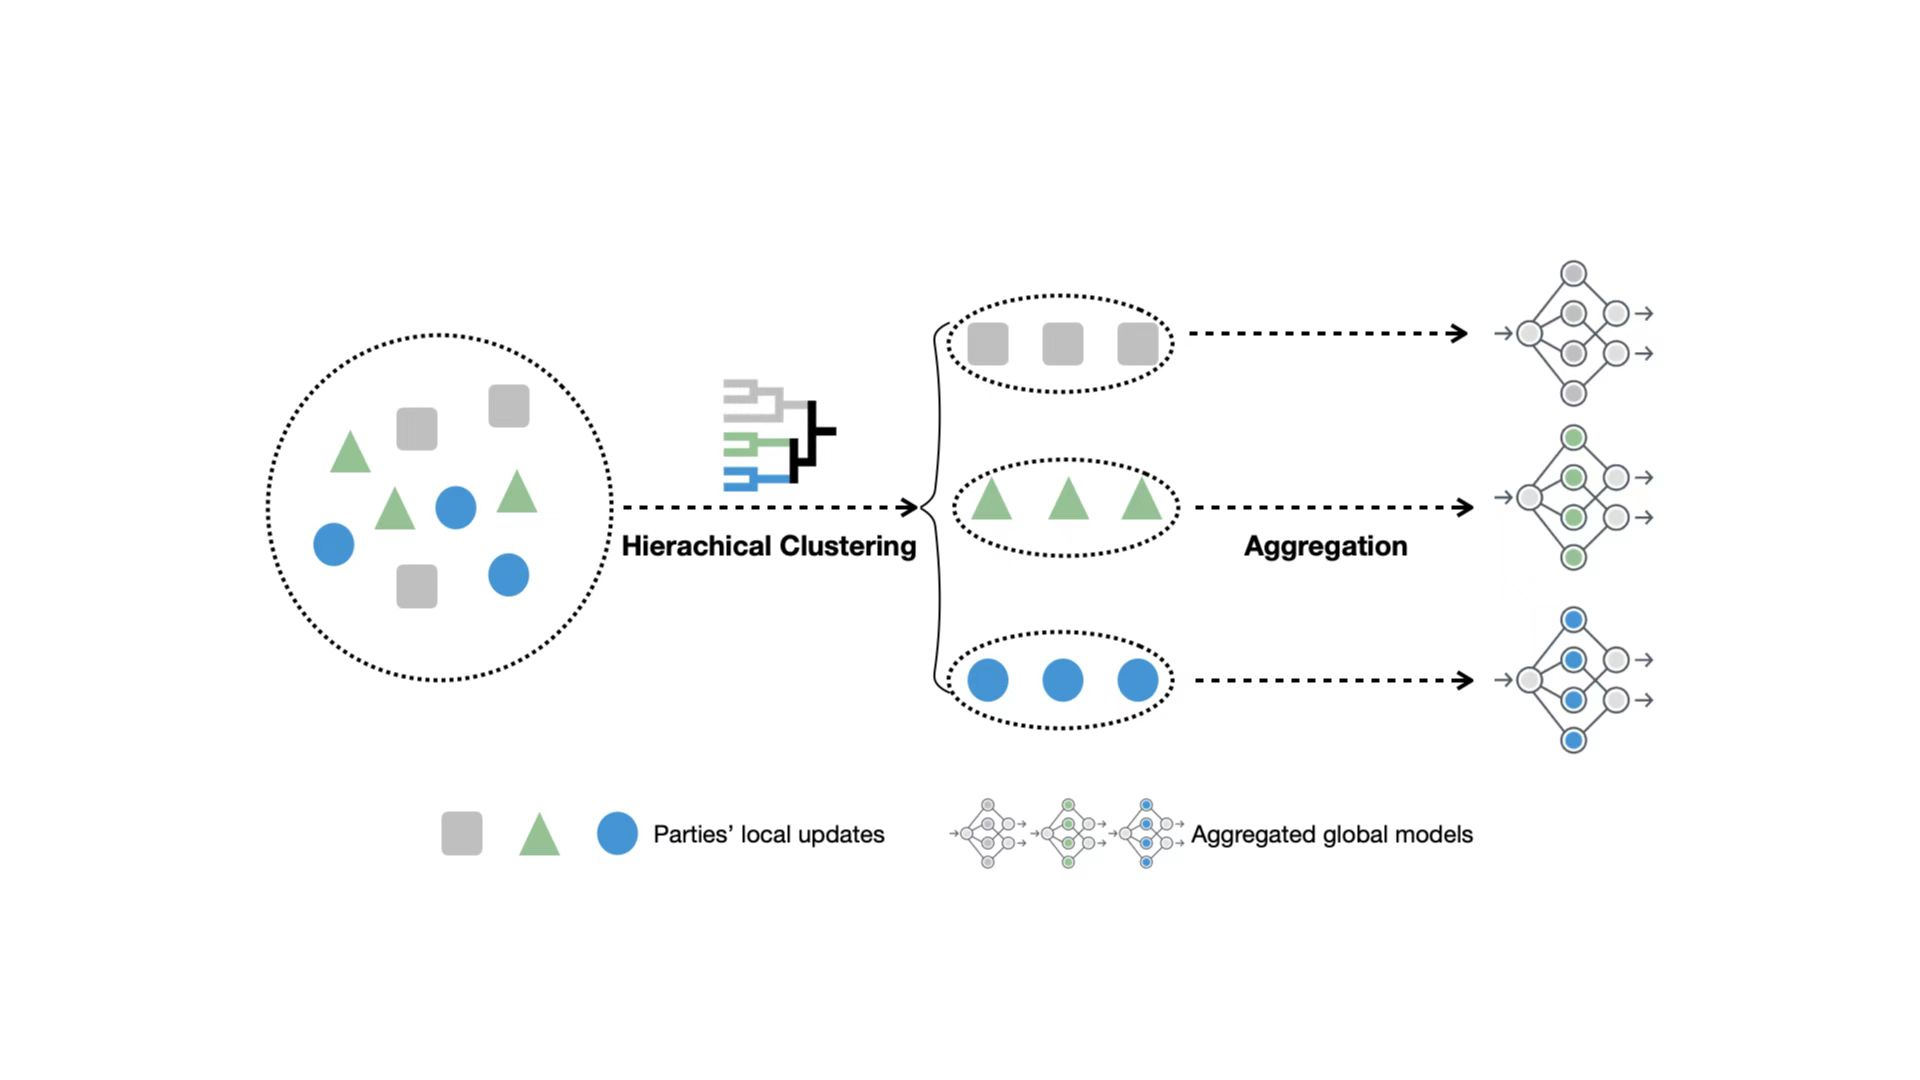
\includegraphics[scale=0.13]{figures/work2figs/hc.jpg}
        \caption{FL+HC简介}
        \label{hcjpg}
    \end{center}
\end{figure}

\subsection{密码技术介绍}

\subsubsection{加性秘密共享}
加性秘密共享是Shamir \cite{shamir1979share} 提出的一种安全多方计算技术。本章我们使用的是一种(2,2)的加性秘密共享方案,可用于安全两方计算(2PC)。这种方案可以在不同大小的环上做两方的安全计算,本章使用到的是两种特殊的环,环$\mathbb{Z}_2$和$\mathbb{p}, p=2^l$($l$一般为32)。当使用环$\mathbb{Z}_2$时,也被称为布尔秘密共享。
在布尔秘密共享方案中,布尔值$x \in \mathbb{Z}_2$可以被拆分为布尔共享份$\langle x\rangle_0^B$ 和 $\langle x\rangle_1^B$,其中三者满足$x = \langle x\rangle_0^B \oplus \langle x\rangle_0^B\;\text{mod}\;2$。
在使用环$x \in \mathbb{Z}_p$时,可以把环$\mathbb{Z}_p$上的元素$x$拆分为两个共享份$(\langle x\rangle_0, \langle x\rangle_1) = (r, x -r) \in \mathbb{Z}_p^2$, 其中$r$是在环$\mathbb{Z}_p$上随机采样得到的元素。通过执行安全的两方计算协议 \cite{rathee2020cryptflow2, rathee2021sirnn},在不重构出原始值的情况下,完成任意的算术运算。

\subsubsection{本章使用的安全两方计算(2PC)协议}
为了在共享份额上进行进行安全的计算,我们使用到了三种加性秘密共享上的基本运算 \cite{rathee2021sirnn},其基本信息的描述如下:
\begin{compactitem}
    \item \textbf{安全两方有符号数乘法}(Signed Value Multiplication,$\mathcal{F}_{\text{SMul}}$): 有符号数乘法 $(\mathcal{F}_{\text{SMul}})$ 以两方上的共享份额 $\langle x\rangle$ 以及 $\langle y\rangle$ 作为输入,然后输出 $\langle z\rangle$,其中三者满足:$z = x \times y$。
    \item \textbf{安全两方多路选择器}(Multiplexer,$\mathcal{F}_{\text{MUX}}$): 多路选择器 $(\mathcal{F}_{\text{MUX}})$ 以 $\langle x\rangle^B$ 和 $\langle y\rangle$ 作为输入,然后输出 $\langle z\rangle$,其中如果$x = 1$,则输出的$z$满足$z = y$,否则满足$z = 0$。 
    \item \textbf{安全两方DRelu} $(\mathcal{F}_{\text{DRelu}})$: DRelu 函数 $(\mathcal{F}_{\text{DRelu}})$ 以 $\langle x\rangle$ 作为输入,然后输出 $\langle z\rangle^B$,其中如果$x \geq 0$,则输出的$z$满足 $z = 1$,否则满足 $z = 0$。
\end{compactitem}

\subsubsection{伪随机生成技术}
伪随机生成技术(Pseudorandom Generator, PRG)\cite{yao1982theory} 可以根据一个均匀分布的随机数种子,生成一串很长的伪随机字符。只要这个随机数种子不被敌对方窃取,就能保证生成的这段随机字符,无法在多项式时间内与均匀分布采样出来的字符串做出区分。本章方案使用伪随机生成技术在参数上传和分发阶段保证参数隐私的同时,减少一半的通信开销(细节见\ref{4-framwork})。

\section{问题描述}\label{4-problem}

\section{基于秘密共享的隐私保护计算模块}\label{4-building}

\section{面向异质数据的隐私保护梯度聚合方案}\label{4-framework}

\section{实验评估}\label{4-exp}

\section{本章小结}\label{4-conclusion}